\section{Introduction}

\begin{figure}
    \centering
    \vspace{1cm}
    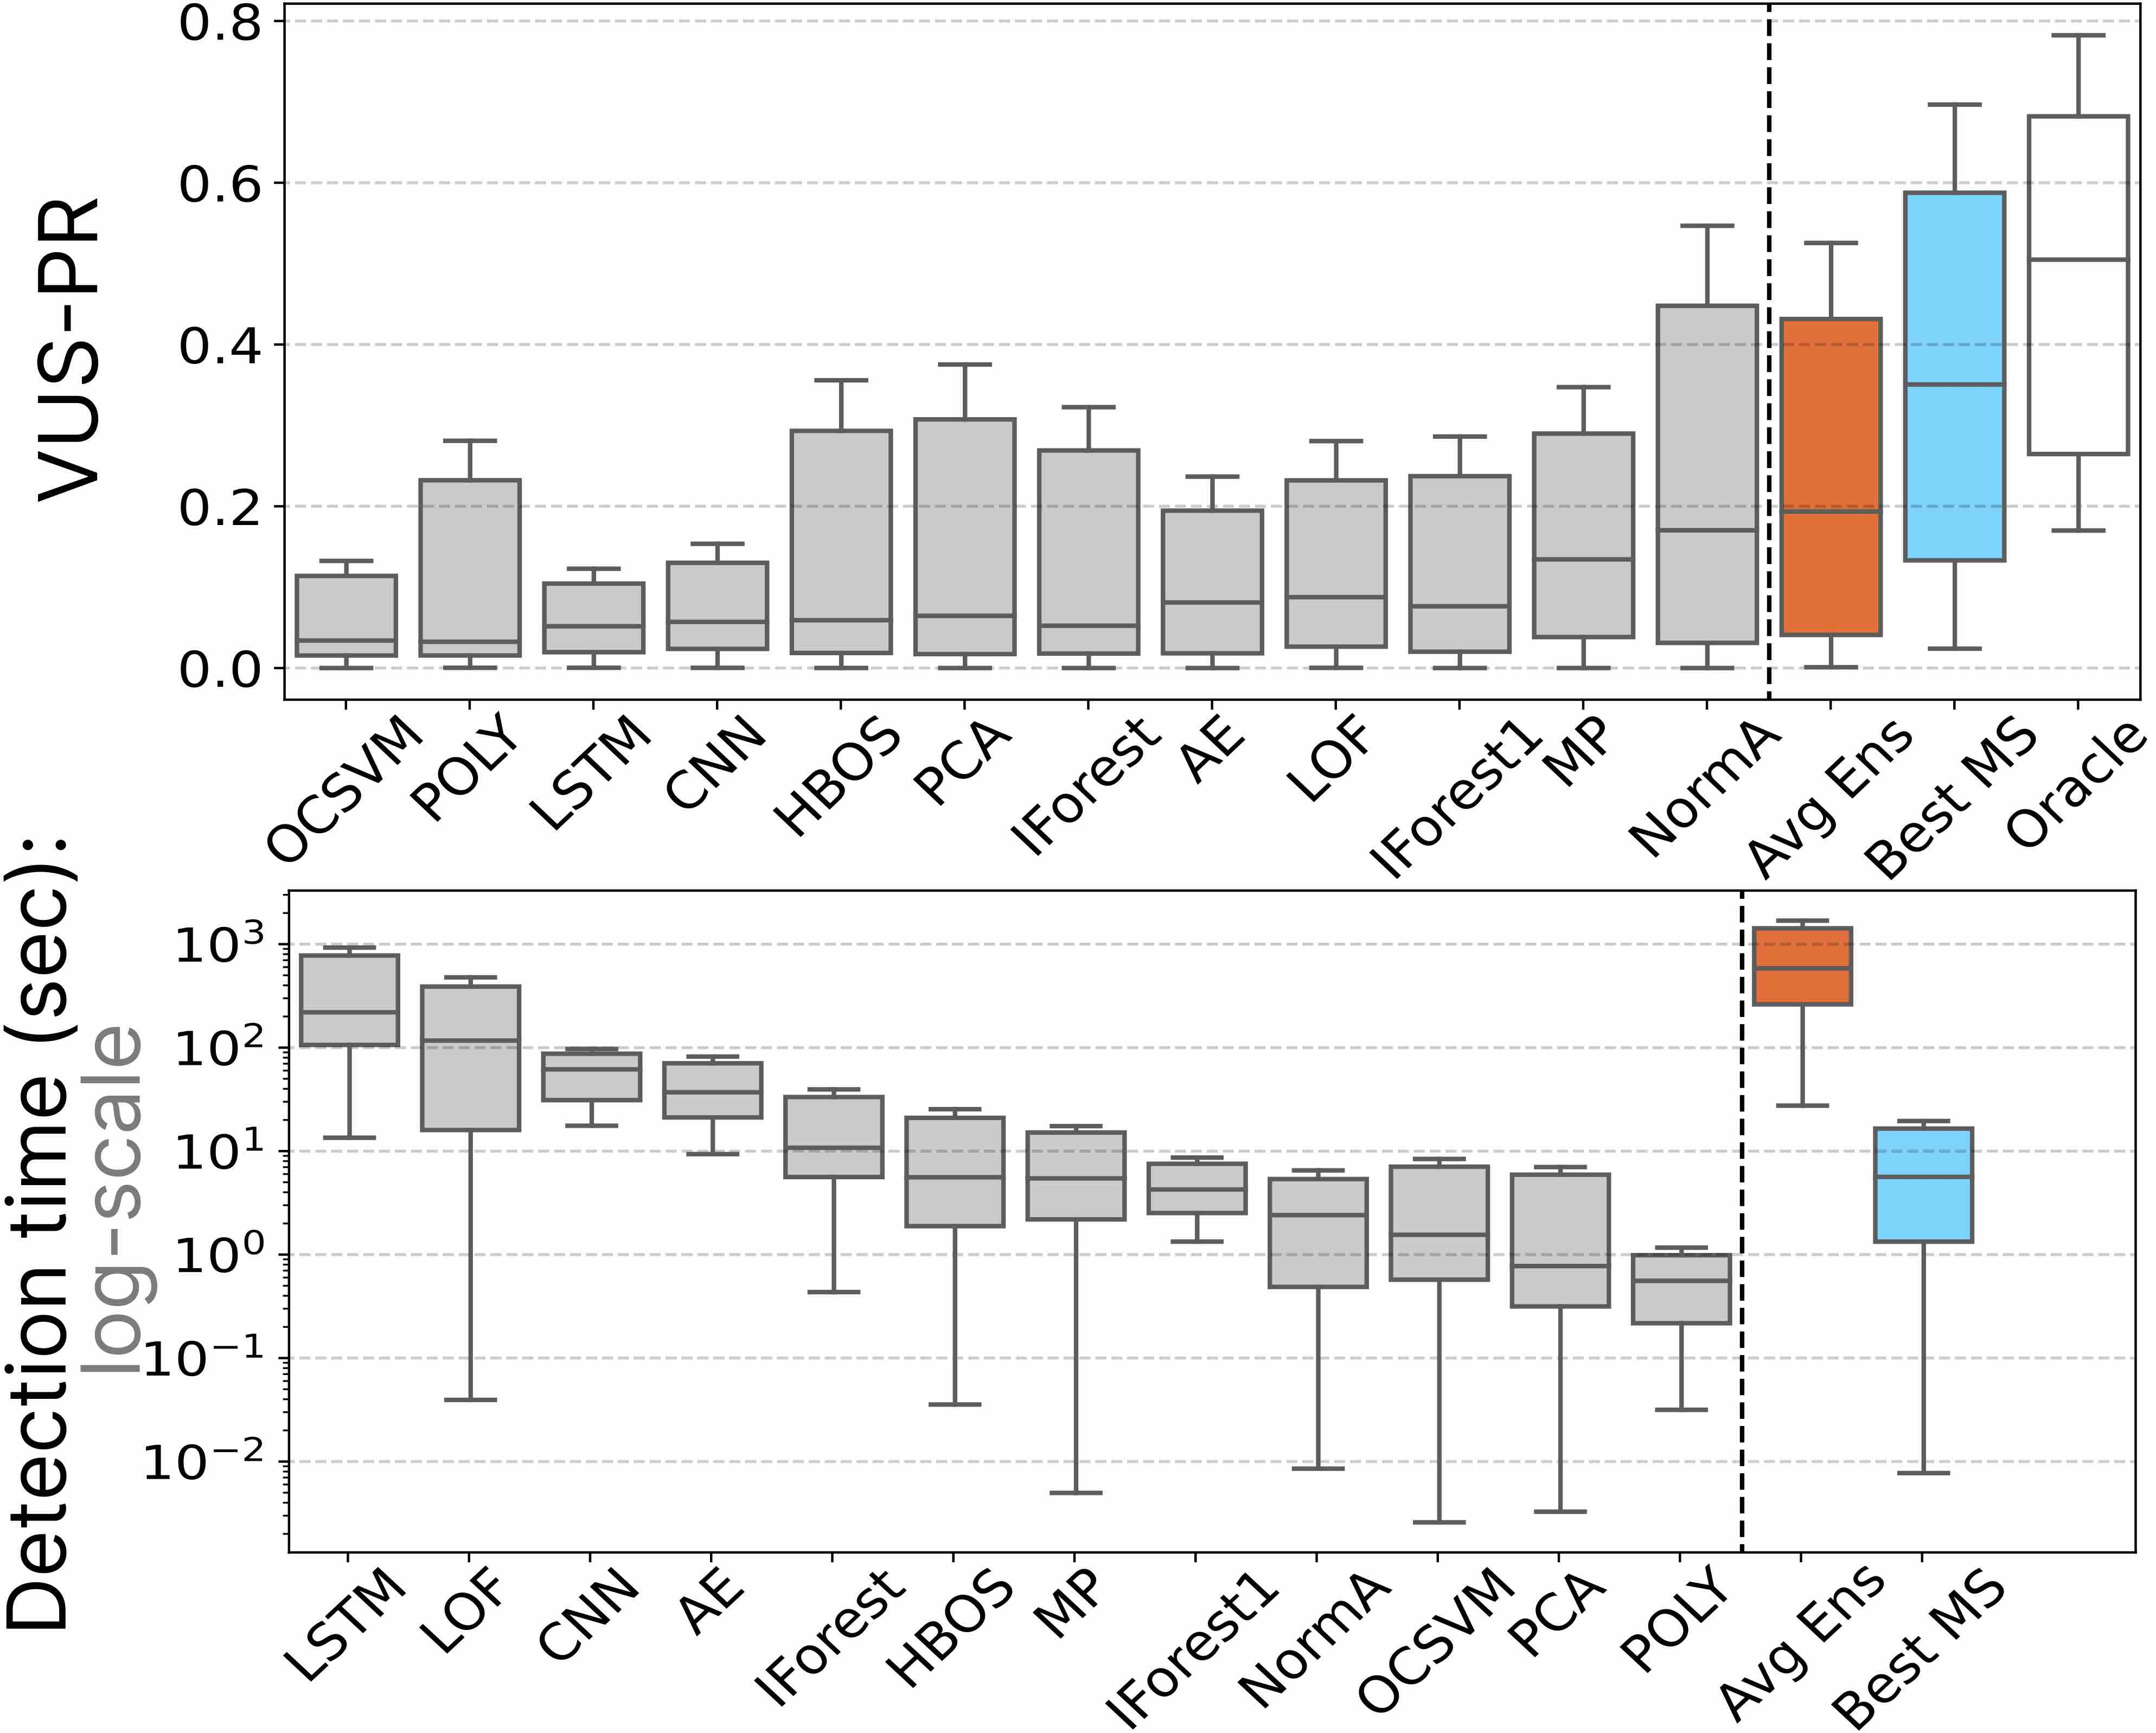
\includegraphics[width=0.82\linewidth]{figures/1_intro_fig.jpg}
    \vspace{-0.3cm}
    \caption{Summary of our evaluation on the TSB-UAD benchmark ~\cite{10.14778/3529337.3529354} of model selection methods (best in blue) when compared to 12 anomaly detection methods and the Avg Ens (in orange).}
    \vspace{-0.3cm}
    \label{fig:intro_fig}
\end{figure}

%large quantity of time series

Extensive collections of time-dependent measurements are a reality in every scientific domain ~\cite{Palpanas2015,DBLP:journals/dagstuhl-reports/BagnallCPZ19, Palpanas2019, paparrizos2021vergedb, liu2023amir,paparrizos2018fastthesis}. 
The recording of these measurements results in an ordered sequence of real-valued data points, commonly referred to as {\em time series} \cite{paparrizos2015k,paparrizos2017fast,bariya2021k,paparrizos2022fast,paparrizos2023accelerating}. 
Analyzing time series data is becoming increasingly important in virtually every scientific and industrial domain \cite{DBLP:conf/edbt/EchihabiZP21,DBLP:journals/pvldb/EchihabiPZ21,liu2021decomposed,jiang2020pids,jiang2021good,dziedzic2019band,paparrizos2019grail,paparrizos2020debunking,paparrizos2016detecting,paparrizos2016screening,mckeown2016predicting,goel2016social,DBLP:journals/pvldb/0003WNP22,DBLP:conf/eenergy/PetraliaCBP23}. 
%, including astronomy~\cite{huijse2014computational}, biology~\cite{bar2003continuous}, %economics~\cite{lutkepohl2004applied}, 
%energy sciences~\cite{bach2017flexible}, 
%engineering~\cite{uehara2002extraction}, 
%environmental sciences \cite{goddard2003geospatial}, medicine~\cite{richman2000physiological}, %neuroscience~\cite{biswal2010toward}, 
%and social sciences~\cite{brockwell2016introduction}.
Anomaly detection, in particular, has received ample academic and industrial attention~\cite{page1957problems,fox1972outliers}, %and has become a significant problem that finds 
finding applications across a wide range of domains and situations. These applications share the same goal~\cite{statisticaloutliers, DBLP:conf/vldb/SubramaniamPPKG06, DBLP:conf/icdm/YehZUBDDSMK16}: analyzing time series to identify observations that do not correspond to %an 
expected behavior. % inferred from previously observed data. 
In practice, anomalies can correspond to~\cite{aggarwal2017introduction}: (i) noise or erroneous data (e.g., broken sensors); or (ii) actual data of interest (e.g., abnormal behavior of the observed system). In both cases, detecting such types is crucial for many applications~\cite{IMSGroundtruth, DBLP:conf/healthcom/HadjemNK16}.


In recent years, many techniques have been proposed for time-series anomaly detection. Multiple surveys and benchmarks summarize and analyze the state-of-the-art proposed methods~\cite{blazquez2021review,10.14778/3529337.3529354,10.14778/3538598.3538602,10.14778/3551793.3551830,10.14778/3476249.3476307,wu2020current,7424283,jacob2020exathlon,Kim2021TowardsAR}. Such surveys and benchmarks provide a holistic view of anomaly detection methods and how they perform. Unfortunately, these benchmark and evaluation studies demonstrated that no overall best anomaly detection methods exist when applied to very heterogeneous time series (i.e., coming from very different domains). In practice, we observe that some methods outperform others on specific time series with either specific characteristics (e.g., stationary or non-stationary time series) or anomalies (e.g., point-based or sequence-based anomalies). 


To overcome the above limitation, ensembling solutions have been proposed~\cite{10.1145/2830544.2830549} that consist of running all existing anomaly detection methods and averaging all anomaly scores. Figure~\ref{fig:intro_fig} shows that this solution (in orange) is outperforming all individual existing techniques in the TSB-UAD benchmark~\cite{10.14778/3529337.3529354,boniol2022theseus}. Nevertheless, as shown in Figure~\ref{fig:intro_fig}, such solutions require running all methods, resulting in an excessive cost that is not feasible in practice.

Therefore, the only scalable and viable solution to solve anomaly detection over very different time series %collected from various domains 
is to propose a model selection method that will select, based on time series characteristics, the best anomaly detection method to run. This topic has been tackled in several recent research works related to AutoML (Automated Machine Learning) for the general case of anomaly detection~\cite{NEURIPS2021_23c89427, https://doi.org/10.48550/arxiv.2009.04395}. %and also for time series~\cite{https://doi.org/10.48550/arxiv.2009.04395,https://doi.org/10.48550/arxiv.2210.01078}. 
Nevertheless, existing AutoML solutions require (i) a universal objective function among models, which is not applicable to anomaly detection methods; (ii) a predefined set of features, which is difficult to obtain for time series due to varying lengths and the lack of standardized featurization solutions; (iii) running multiple anomaly detection methods several times, which is prohibitively expensive in practice; or (iv) labeled anomalies, which (in contrast to classification tasks) are difficult to obtain. Therefore, more work is needed in order to render AutoML solutions applicable to time-series anomaly detection. 


The objective is to train a time series classification model on time series for which we know in advance which anomaly detection method is the best. However, the lack of a benchmark with labeled time series has been a limiting factor for training robust model selection models (this only changed very recently~\cite{10.14778/3529337.3529354,10.14778/3538598.3538602,kdd21}). Therefore, there exists no experimental evaluation that measures the effectiveness of classification methods for the task of model selection for time series anomaly detection. Though, such an evaluation is very important for determining which time series classification methods are accurate as model selection methods, and which solutions should be considered in unsupervised settings (i.e., using model selection approaches on time series from domains that were not included in the training set). These results would help the design and effectiveness of general AutoML pipelines for time series.

Thus, in this paper, we evaluate the performance of time series classification methods used as model selection for anomaly detection in time series. To do so, we propose a pipeline that enables any kind of time series classifier to be used for any univariate time series with different lengths. We then compare the execution time and accuracy for feature-based, traditional time series classifiers and deep learning classification algorithms. We also measure how these models perform when trained on time series of a given domain (e.g., electrocardiogram~\cite{Moody}) and tested on time series from a different domain (e.g., robotics sensors measurements~\cite{5573462}). 

Overall, we compare \syl{16} different classifiers over 1980 time series and 12 anomaly detection methods from the recent anomaly detection benchmark TSB-UAD. Thus, we propose the first extensive experimental evaluation of time series classification as model selection for anomaly detection. Our results demonstrate that model selection methods outperform every single anomaly detection method while being in the same order of magnitude regarding execution time. Figure~\ref{fig:intro_fig} shows a summary of our experimental evaluation, where the best model selection method (in blue in Figure~\ref{fig:intro_fig}) is up to 2.8$\times$ more accurate than the best anomaly detection method in the TSB-UAD benchmark and 1.9$\times$ more accurate than the ensembling solution mentioned above. This evaluation is the first step to demonstrate the accuracy and efficiency of time series classification algorithms for anomaly detection. It represents a strong baseline that can then be used to guide the choice of approaches for the model selection step in more general AutoML pipelines.

%We start with a detailed discussion of the relevant background and related work for anomaly detection in time series (Section~\ref{sec:background}). Then, we present our contributions:
Our contributions can be summarized as follows\syl{:}
\begin{itemize}[noitemsep, topsep=0pt, parsep=0pt, partopsep=0pt, leftmargin=0.4cm]
	\item We cast the model selection problem for time-series anomaly detection methods into a time-series classification problem. We describe and study the need to evaluate time series classification methods for model selection (Section~\ref{sec:problem_def}). 
	\item We introduce our novel pipeline for model selection applied to anomaly detection in time series. As this pipeline is generic, we describe how it can be used with both feature-based classification methods, traditional time series classification methods, and deep learning-based methods (Section~\ref{sec:proposed}).
	\item We describe our experimental framework (on top of the recent anomaly detection benchmark TSB-UAD~\cite{10.14778/3529337.3529354}), and provide details on both anomaly detection methods and time series classification methods considered in this paper (Section~\ref{sec:exp}). We make all our material publicly available online~\cite{ourcode} and provide an interactive WebApp~\cite{ourwebsite} for exploring our results. 
	\item We present an extensive experimental evaluation, measuring the anomaly detection accuracy and execution time (both training and inference) of model selection algorithms (Section~\ref{exp:overalleval}). We evaluate the influence of important parameters and the relationship between classification and anomaly detection accuracy (Sections~\ref{exp:windowlength}, \ref{exp:datasets}, and \ref{exp:detectionvsclass}). Moreover, we measure the transferability of model selection algorithms to new types of time series by testing multiple combinations of train and test datasets that do not contain the same kinds of time series (Section~\ref{exp:sup2unsup}).
\end{itemize}
Finally, we conclude with the implications of our work and discuss possible future directions that could help improve both the accuracy and the execution time of our proposed pipeline (Section~\ref{sec:conclusions}).